\chapter{Badania}

\section{Przeprowadzone badania}

Zgodnie z założeniami, badania przeprowadzono dla 5 różnych liczb neuronów w warstwie ukrytej: \textbf{5, 10, 20, 40, 60}. W celu uzyskania możliwie jak najdokładniejszych wyników, każdy eksperyment powtórzono 5 razy, zaś wyniki uśredniono i wraz z wyliczonym odchyleniem standardowym, zaprezentowano na wykresach. Pojedynczy eksperyment składa się z następujących kroków:

\begin{enumerate}[noitemsep]
	\item{Wybranie rozmiaru warstwy ukrytej.}
	\item{Wybranie liczby cech.}
	\item{Przeprowadzenie 10-krotnej walidacji krzyżowej, na którą składa się}
	\begin{enumerate}
		\item{Podział zbioru na podzbiory uczący oraz testujący.}
		\item{Wybranie najlepszych cech.}
		\item{Nauczenie klasyfikatora.}
		\item{Ocena jakości klasyfikacji.}
	\end{enumerate}
	\item{Uśrednienie wyników.}
	\item{Prezentacja wyników.}
\end{enumerate}

Parametry, których użyto w badaniach znajdują się w tabeli \ref{tab:params}.

\begin{table}[h!]
    \centering
    \caption{Parametry algorytmów.}
    \label{tab:params}
    \begin{tabular}{p{3cm}p{3cm}p{9cm}}
        \toprule
        \textbf{Parametr} & \textbf{Wartość} & \textbf{Opis} \\
        \midrule
        \texttt{algorithm} & \texttt{sgd} & Algorytm działania (\textit{stochastic gradient descent}). \\
        \texttt{max\_iter} & \texttt{10000} & Maksymalna liczba iteracji. \\
        \texttt{alpha} & \texttt{1e-6} & Parametr regularyzacji. \\
        \texttt{learning\_rate} & \texttt{constant} & Tempo uczenia. \\
        \texttt{activation} & \texttt{logistic} & Funkcja aktywacji algorytmu \texttt{BP}. \\
        \texttt{activation} & \texttt{multiquadric} & Funkcja aktywacji algorytmu \texttt{ELM}. \\
        \bottomrule
    \end{tabular}
\end{table}

\section{Porównanie algorytmów}

Dla 5 neuronów w warstwie ukrytej można zauważyć, że oba algorytmy osiągnęły prawie takie same wyniki oscylujące w okolicy 76\%, niezależne od liczby wyselekcjonowanych cech.

Również czasy wykonywania klasyfikacji okazały się bardzo podobne.
Wystąpiły tutaj jednak większe fluktuacje, spowodowane przede wszystkim niedokładnością w mierzeniu bardzo małych czasów (rzędu 0.5 milisekundy) oraz dużym odchyleniem standardowym sygnalizowanym na wykresie przez słupki błędu.

Największą różnicę zauważyć jednak można w średnich czasach uczenia -- 2ms dla \texttt{ELM} i 130ms dla sieci neuronowej.

\begin{figure}[h!]
	\centering
	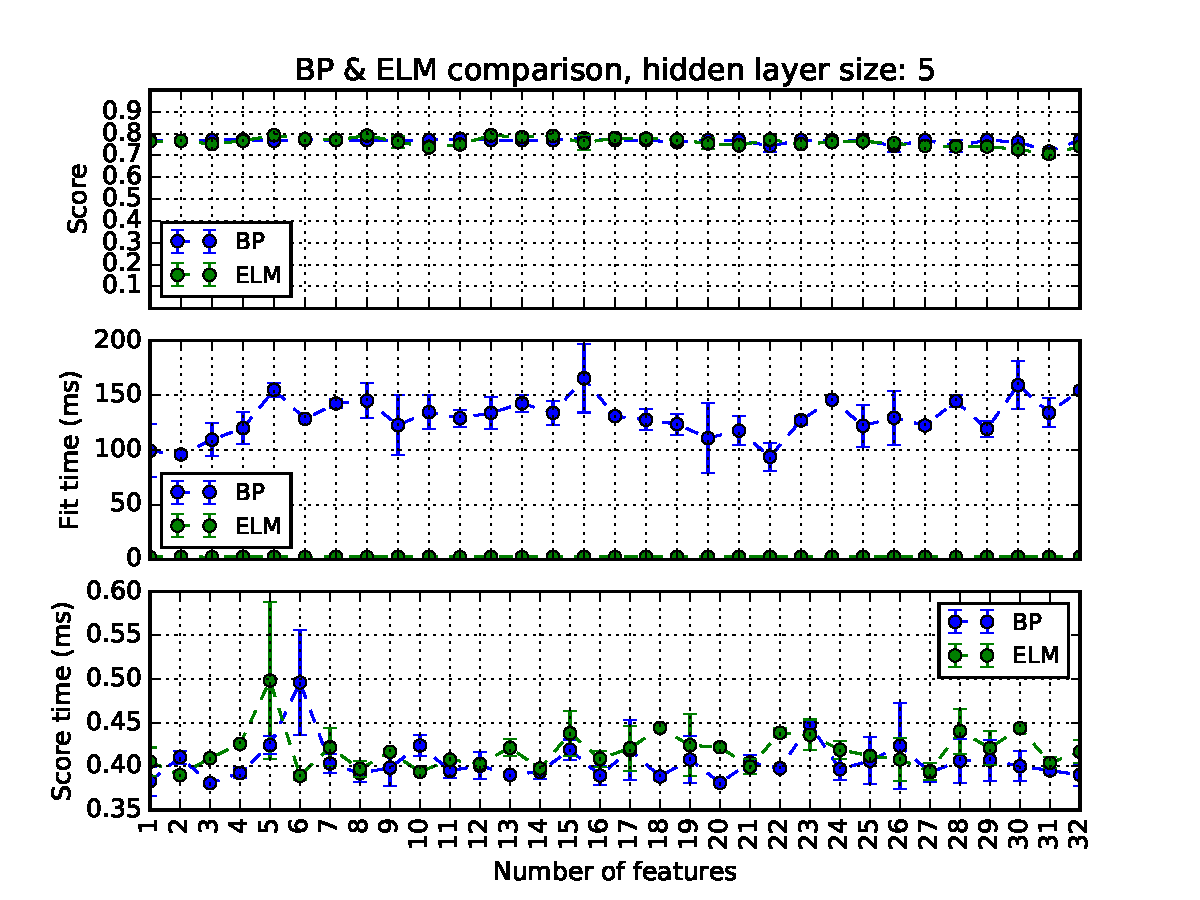
\includegraphics[width=1.0\linewidth]{img/bp_elm_5.pdf}
	\label{Rysunek}
	\caption{5 neuronów w warstwie ukrytej - porównanie obu algorytmów}
\end{figure}

\newpage

Dla 10 neuronów w warstwie ukrytej zachodzą te same zależności. Widoczny jest jednak nieznaczny wzrost czasu uczenia dla algorytmu \texttt{BP} do około 250 milisekund w okolicy 10-14 wyselekcjonowanych cech. Algorytm \texttt{ELM} pozostaje bez zmian.

\begin{figure}[h!]
	\centering
	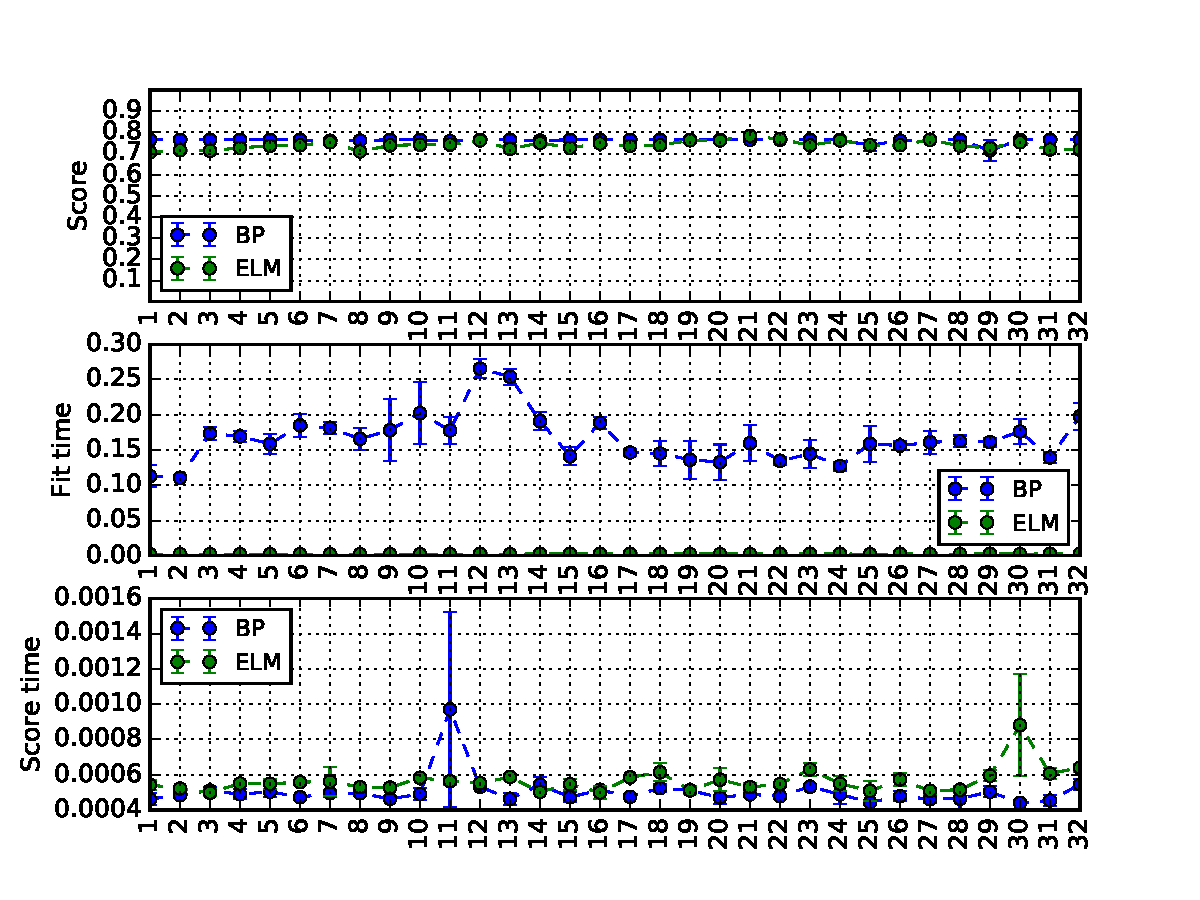
\includegraphics[width=1.0\linewidth]{img/bp_elm_10.pdf}
	\label{Rysunek}
	\caption{10 neuronów w warstwie ukrytej - porównanie obu algorytmów}
\end{figure}

\newpage

Dla 20 neuronów w warstwie ukrytej zdecydowanie zauważyć już można tendencję w czasie uczenia algorytmu \texttt{BP}, gdzie do około 7 wyselekcjonowanych cech czas znacząco wzrasta, później do około 16 cech pozostaje względnie stały, następnie maleje i od 22 cech utrzymuje się już na stałym, niskim poziomie rzędu 100 milisekund. Wytłumaczyć tę zależność można zjawiskiem przeuczenia, gdzie algorytm osiągnął lokalne minima, a następnie je wykorzystywał przy kolejnych uczeniach.

\begin{figure}[h!]
	\centering
	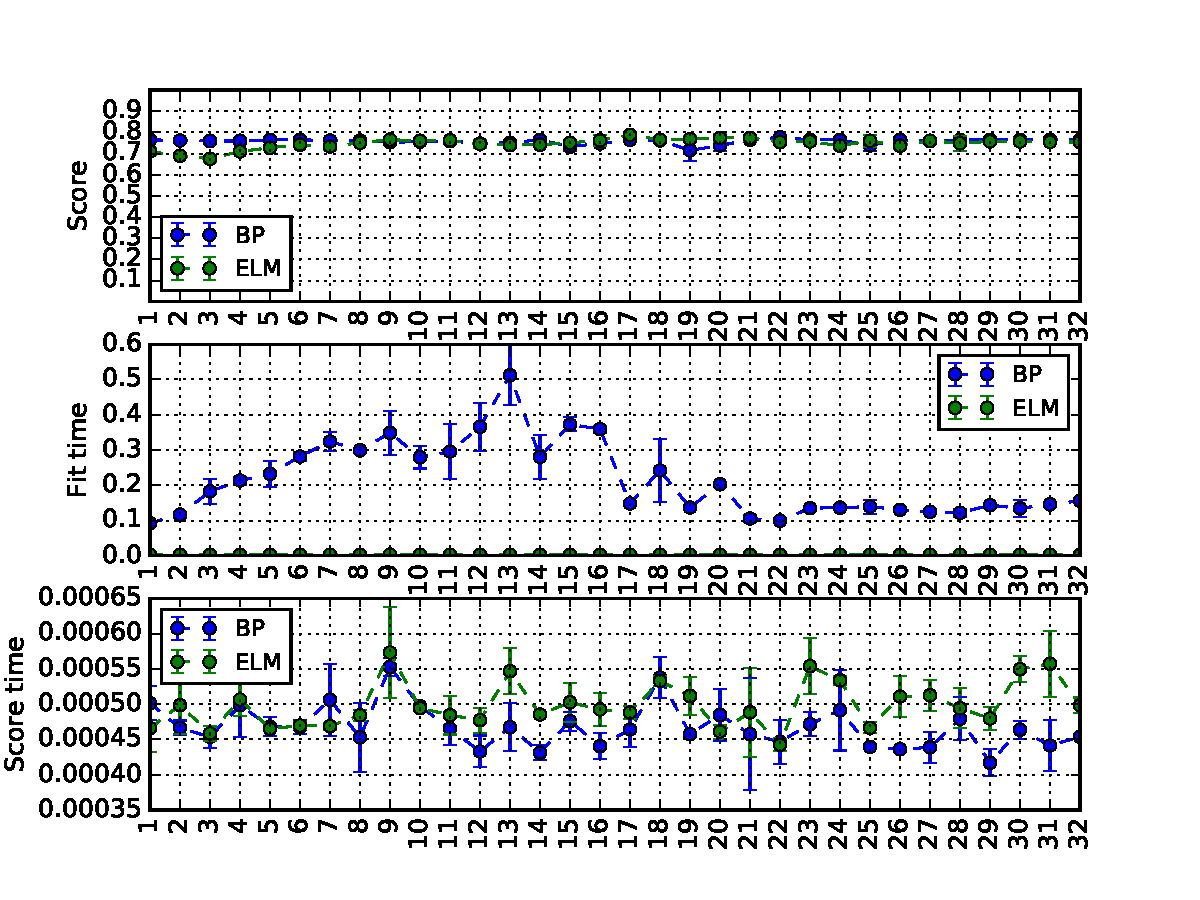
\includegraphics[width=1.0\linewidth]{img/bp_elm_20.pdf}
	\label{Rysunek}
	\caption{20 neuronów w warstwie ukrytej - porównanie obu algorytmów}
\end{figure}

\newpage

Dla 40 oraz 60 neuronów w warstwie ukrytej widać już bardzo wyraźnie zauważone wcześniej tendencje dla algorytmu \texttt{BP}. Reszta zależności pozostaje bez zmian.

\begin{figure}[h!]
	\centering
	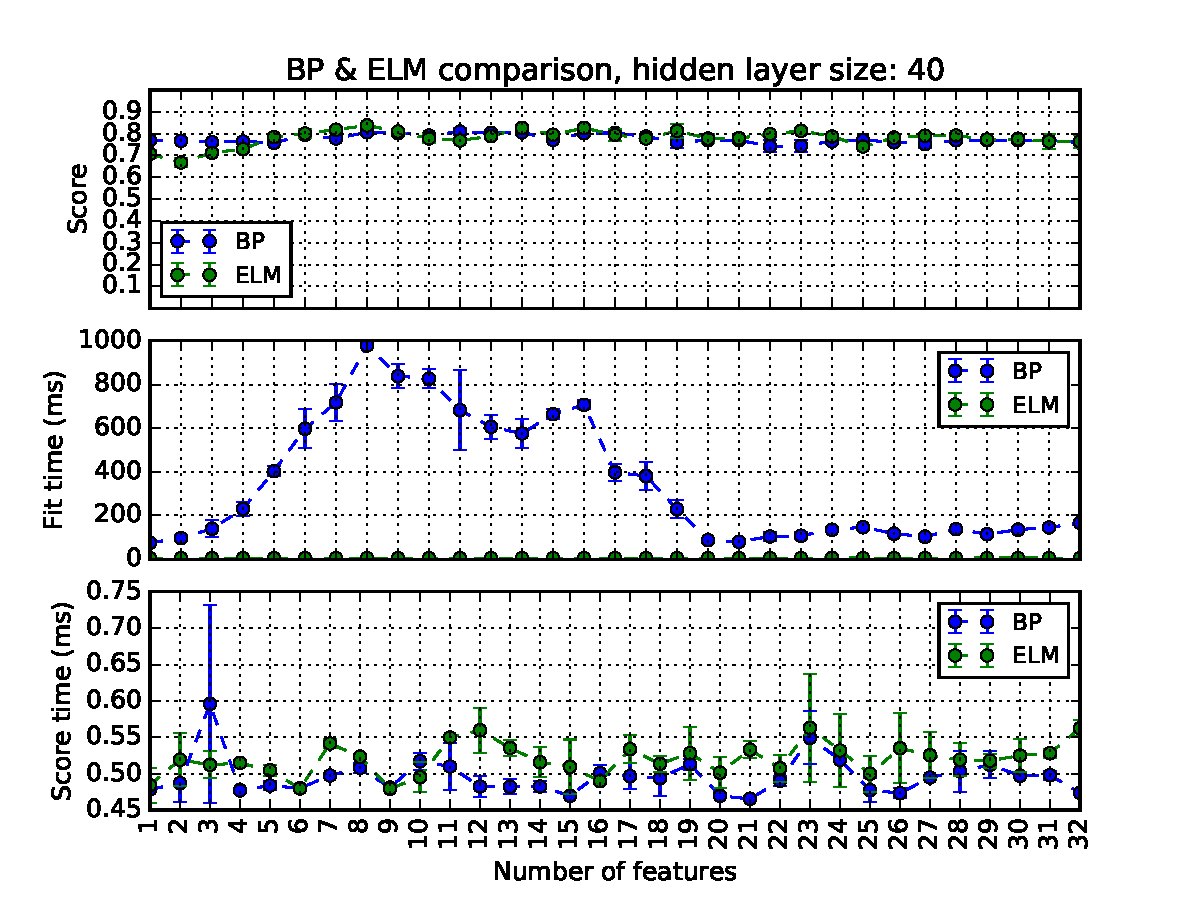
\includegraphics[width=0.78\linewidth]{img/bp_elm_40.pdf}
	\label{Rysunek}
	\caption{40 neuronów w warstwie ukrytej - porównanie obu algorytmów}
\end{figure}

\begin{figure}[h!]
	\centering
	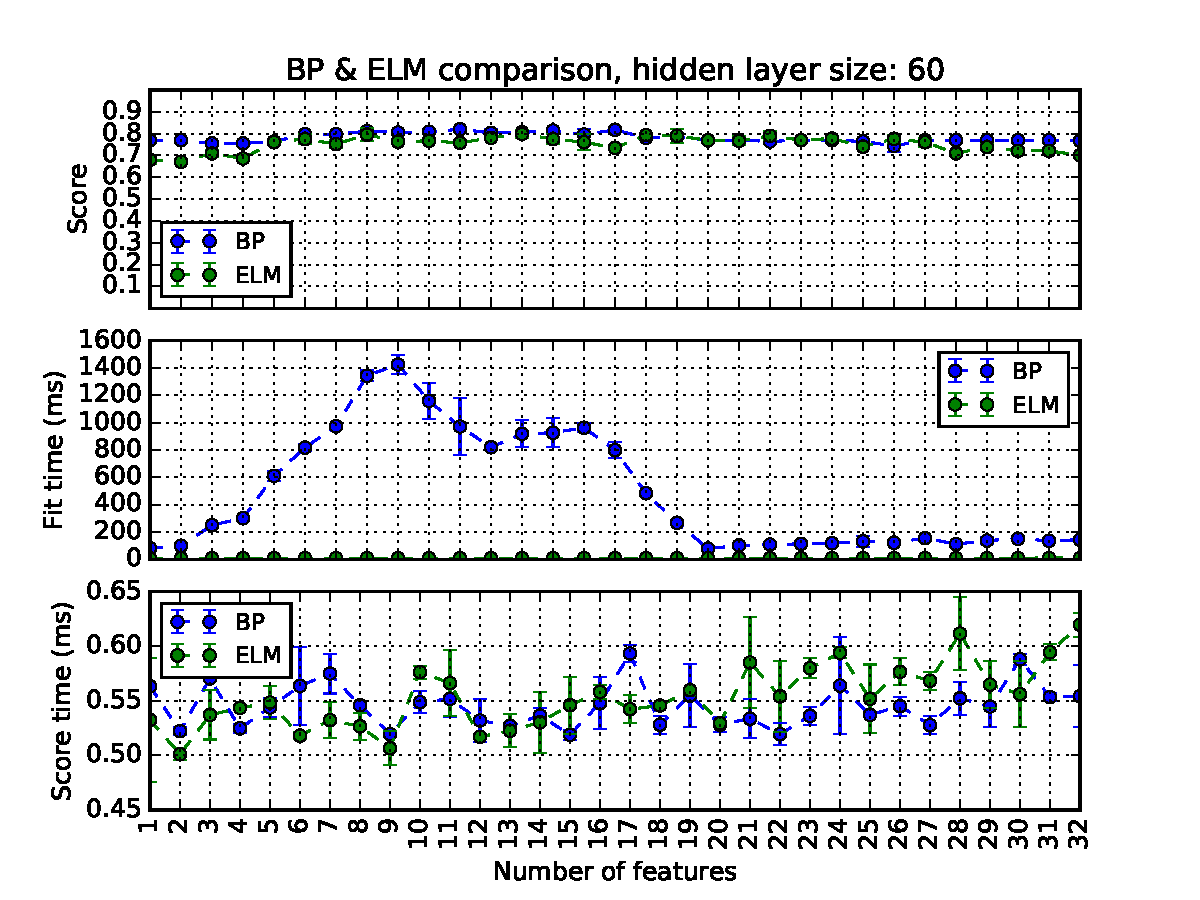
\includegraphics[width=0.78\linewidth]{img/bp_elm_60.pdf}
	\label{Rysunek}
	\caption{60 neuronów w warstwie ukrytej - porównanie obu algorytmów}
\end{figure}

\newpage

\section{Selekcja cech}

Selekcja cech polega na wybieraniu podzbioru cech w celu ograniczenia czasu uczenia, uproszczenia modelu oraz minimalizacji zjawiska przeuczenia.

W projekcie skorzystano z klasy \texttt{SelectKBest}, z modułu \texttt{sklearn.feature\_selection}.

Wykres poniżej przedstawia sumę częstości wybierania cech na przestrzeni wszystkich eksperymentów. Widać wyraźnie, że niektóre cechy wybierane były znacznie częściej niż inne, co oznacza, że były o wiele bardziej przydatne w procesie uczenia algorytmów.

\begin{figure}[h!]
	\centering
	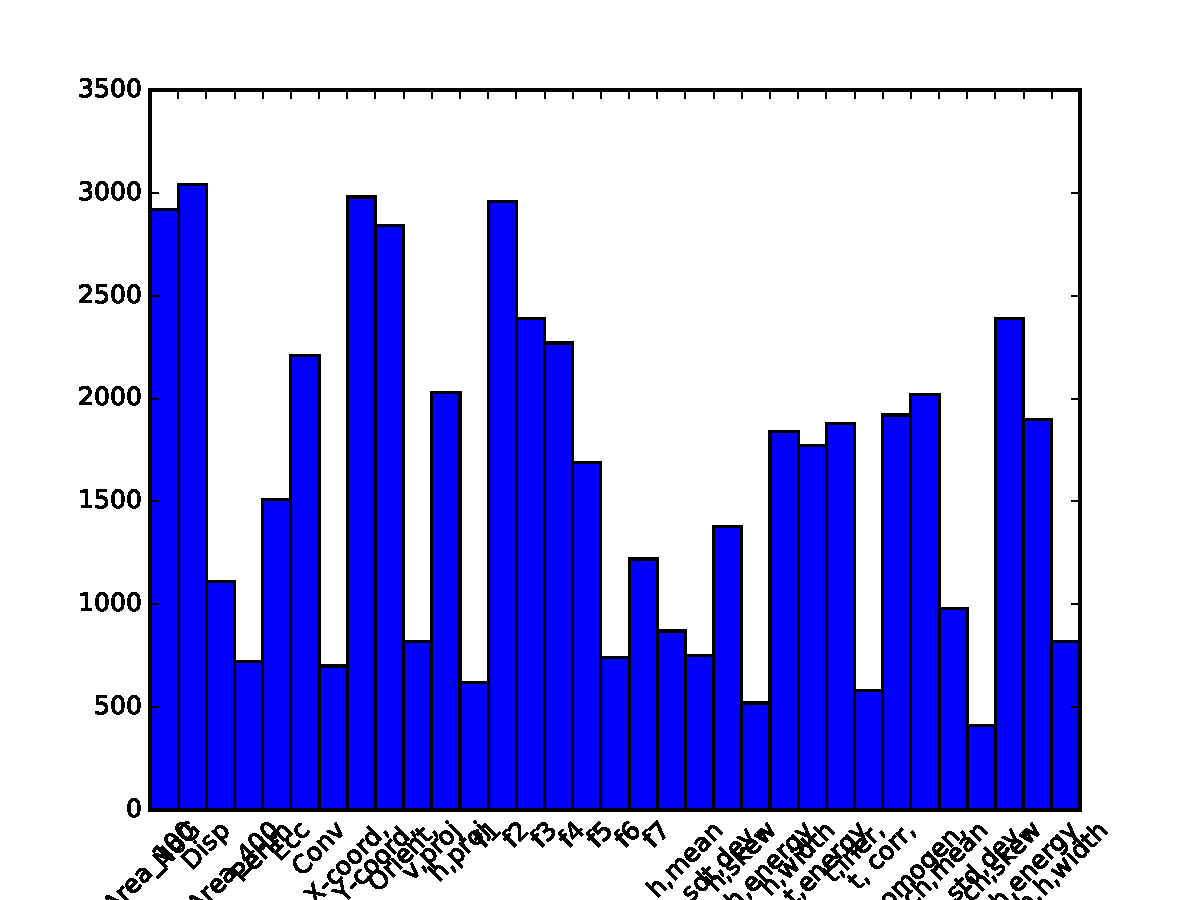
\includegraphics[width=1.0\linewidth]{img/features.pdf}
	\label{selekcja}
	\caption{Częstość wybierania cech}
\end{figure}

\newpage

\section{Macierz pomyłek}

Macierz pomyłek umożliwia zobrazowanie jak dobrze klasyfikator radzi sobie ze swoim zadaniem.

Dla problemu z dwiema klasami -- tak jak w aktualnie rozpatrywanym problemie -- macierz dzieli się na cztery części, w których zliczane są obiekty sklasyfikowane poprawnie -- umieszczone na przekątnej macierzy -- oraz błędnie -- umieszczone poza przekątną.

W projekcie skorzystano z funkcji \texttt{confusion\_matrix}, z modułu \texttt{sklearn.metrics}.

Na przedstawionym rysunku widać wyraźnie, że 14 z badanych obiektów zaklasyfikowanych zostało poprawnie do klasy \texttt{G2}. 4 z nich otrzymało błędną klasyfikację jako \texttt{G2}. Oznacza to, że w tym przypadku algorytm nauczył się klasyfikować wszystkie obiekty do klasy \texttt{G2}, co spowodowane było opisanym wyżej problemem niezbalansowanych danych.

\begin{figure}[h!]
	\centering
	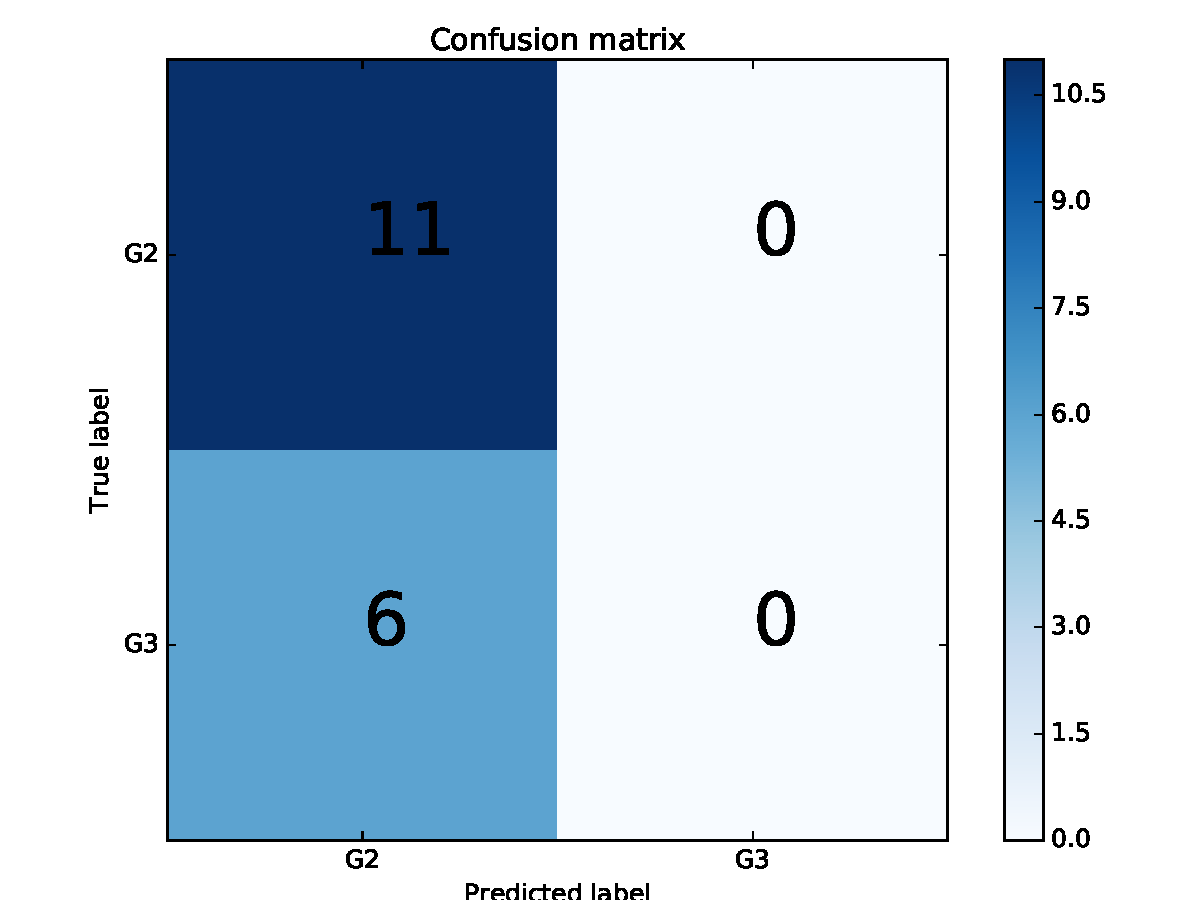
\includegraphics[width=0.8\linewidth]{img/conf_matrix.pdf}
	\label{Rysunek}
	\caption{Przykładowa macierz pomyłek}
\end{figure}
